\documentclass{article}

\usepackage[a4paper, total={6in, 8in}]{geometry}

% SETTINGS %
\usepackage{polski}
\usepackage[utf8]{inputenc}
\usepackage{titlesec}
\usepackage{graphicx}
\usepackage[bookmarks=true,hidelinks]{hyperref}
%  \newcommand{\sectionbreak}{\clearpage}
\newcommand{\documentdate}{21 maja 2018}
\newcommand{\documentversion}{ver. 1.1}

\graphicspath{ {/} }

\title{Fourier's Phone - projekt techniczny}
\author{Frederic Grabowski \and Bartłomiej Karasek \and Wojciech Przybyszewski 
        \and Andrzej Swatowski}
\date{\documentdate \\ \documentversion}

%------------------
% DOCUMENT %
\begin{document}

\maketitle
\newpage

\tableofcontents
\newpage

\section{Opis projektu}
Celem projektu jest zbudowanie aplikacji na telefony z~systemem Android w~wersji
5.0 lub wyższej pozwalającej na przesyłanie różnego rodzaju danych między 
telefonami za pomocą dźwięku.

\section{Wykorzystanie aplikacji}
\vspace{5mm}
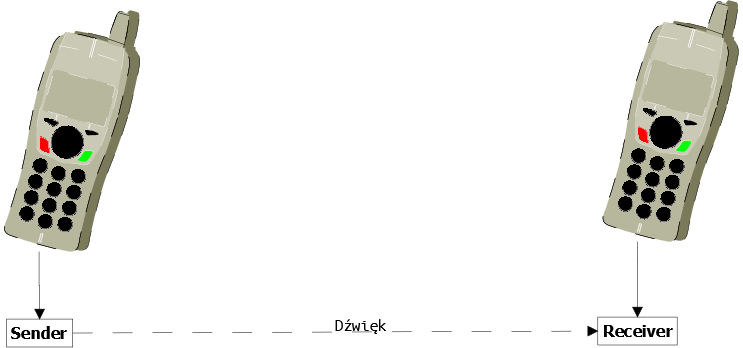
\includegraphics[width=\textwidth]{send_receive_uml.png}
\par
Użytkownicy korzystają z~aplikacji na swoich telefonach z~zainstalowanym
systemem Android w~wersji 5.0 lub wyższej. \par
Zależnie od wybranego trybu (nadawania lub odbierania), aplikacja korzysta
z~odpowiedniej klasy, która to za pomocą zaimplementowanych na niższym poziomie
abstrakcji metod albo wysyła dźwięki o~określonych częstotliwościach, albo je
odbiera. Aplikacja w~trybie odbierania następnie przekształca odebrane dźwięki
w~tekst i~wyświetla na ekranie telefonu.

\section{Architektura aplikacji}
Aplikacja ma jeden ekran, implementowany przez klasę MainActivity, dziedziczącą 
po \textit{AppCompatActivity}. \par
Zależnie od wybranej opcji (za pomocą stosownego przełącznika), MainActivity
korzysta z~metod zaimplementowanych w~klasach Receiver (tryb odbierania) oraz
Sender (tryb nadawania). Klasy te wykorzystują wewnętrzne metody Androida, by
kontrolować mikrofon oraz głośniki. Do tłumaczenia tekstu na dźwięk lub 
odebranych dźwięków na tekst służą publiczne metody \textit{stof} 
i~\textit{ftos} z~klasy Translator. \par
Klasa Receiver korzysta z~klas i~metod umieszczonych w~wewnętrznej paczce
\textit{soundanalyzer}. Wewnętrzna implementacja korzysta z~algorytmów
operujących na dźwiękach i~funkcjach fal, takich jak FFT. \par
Aplikacja oprócz trybu wysyłania tekstu oferuje także tryb wysyłania plików.
Do operacji na plikach zostanie wykorzystana osobna klasa, FileTranslator, która
to oferować będzie publiczne metody \textit{prepareFile} (do wysyłania pliku)
oraz \textit{saveFile} (do tłumaczenia odebranych przez aplikację znaków na
binarną reprezentację pliku). \par
\vspace{5mm}
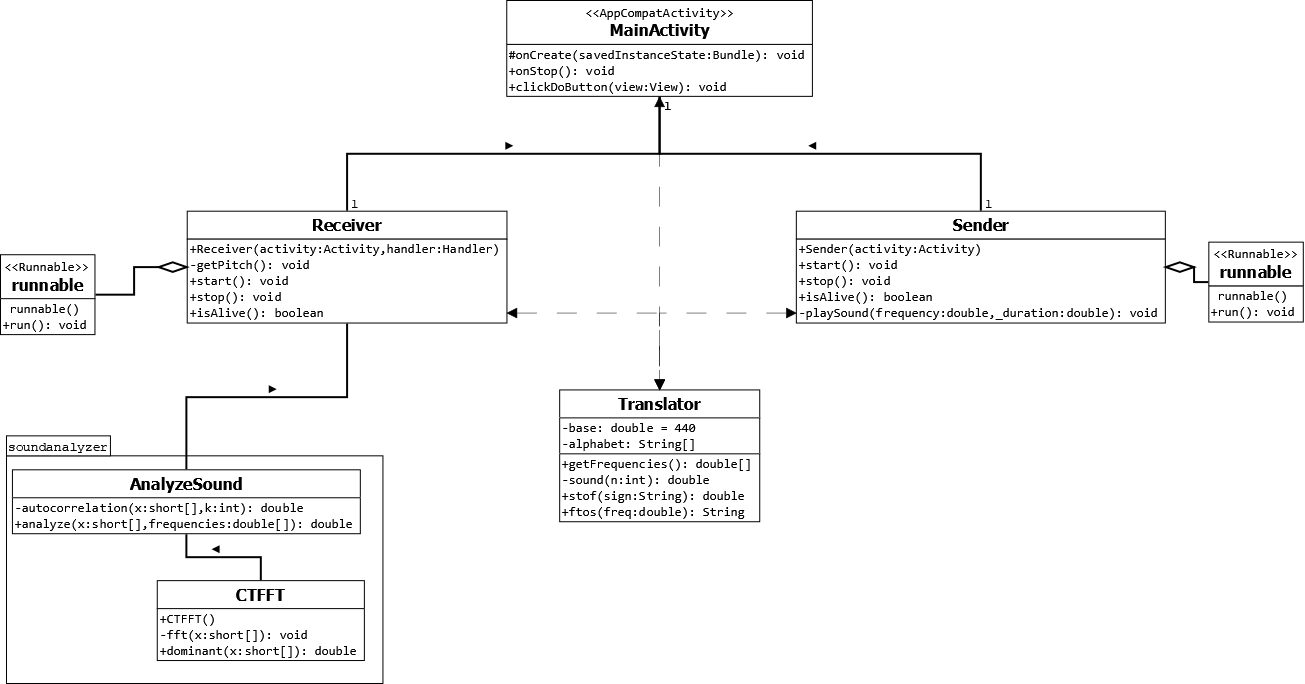
\includegraphics[width=\textwidth]{app_uml.png}

\section{Rozwiązania techniczne/technologie}
Całość aplikacji jest napisana w~Javie, korzystając z~bibliotek systemowych
Androida. Android musi być w~wersji 5.0 lub wyższej, bowiem aplikacja korzysta
z~metod i~funkcjonalności, które pojawiły się dopiero w tej wersji API.

\section{Algorytmy}
W~trosce tak o~wydajność rozwiązania, jak i~poprawność odbieranych danych należy
skorzystać z~odpowiednich algorytmów. \par
Podstawowym algorytmem, z~jakiego aplikacja będzie korzystać (skąd wynika także
jej nazwa) jest FFT - Szybka Transformata Fouriera i~jej najpopularniejsze
implementacje i~modyfikacje (działające chociażby w~$O(n\log{}n)$). \par
Prócz tego zakłada się wykorzystanie innych algorytmów, które przyspieszą
działanie aplikacji oraz zapewnią jej niezawodność lub też radykalnie obniżą
prawdopodobieństwo błędu. Jednym z~takich algorytmów jest autokorelacja.
\end{document}
